\section{Instabilities (89-105)}

\textbf{Motivation:} Navier-Stokes equation in non-dimensional units with no external forces:
\begin{equation}
\pdiff{\vec{v}}{t}+\left(\vec{v}\cdot\vec{\nabla}\right)\vec{v} = -\vec{\nabla}p+\frac{1}{Re}\vec{\nabla}^2\vec{v}
\end{equation}

Reynolds number:
\begin{equation}
Re = \frac{\rho LV}{\mu}=\frac{\rho V^2/L}{\mu V/L^2}=\frac{\mathrm{inertia\ force\ density}}{\mathrm{friction\ force\ density}}
\end{equation}
As the Reynolds number increases, a stable flow becomes unstable, and a new stable flow emerges.

\textbf{Big question:} when does a stable flow become unstable?

Answer: linear stability analysis

\begin{figure}[h]
    \centering
    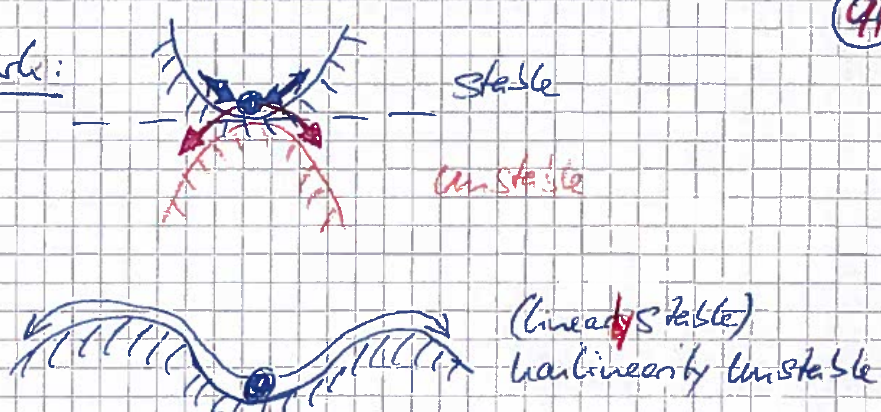
\includegraphics[width=.8\textwidth]{week7/stable-unstable}\\
    \caption{}
    \label{fig:stable-unstable}
\end{figure}


\begin{figure}[p]
    \centering
    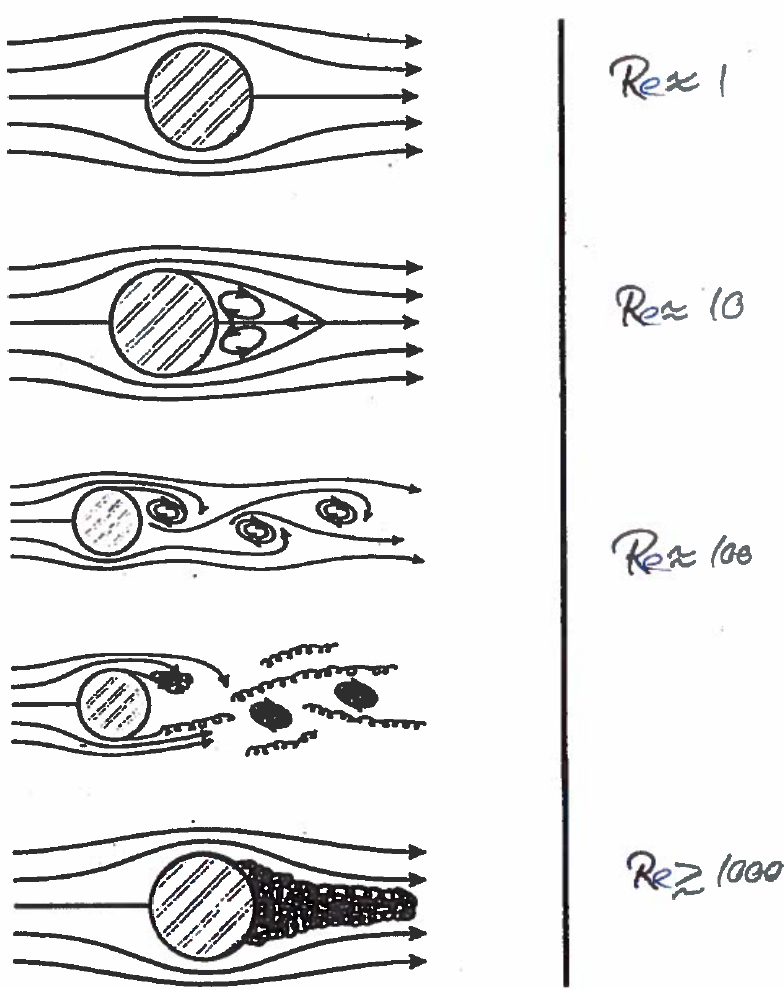
\includegraphics[width=\textwidth]{week7/reynolds-number}\\
    \caption{}
    \label{fig:reynolds-number}
\end{figure}


\textbf{Sketch of linear stability analysis}

Simplifying assumptions: stable flows are steady (stationary)
\begin{equation}
\vec{v}(\vec{r},t)=\vec{U}(\vec{r})\ ,\quad p(\vec{r},t)=P(\vec{r})
\end{equation}

Introduce perturbations
\begin{align}
\vec{v}(\vec{r},t)&=\vec{U}(\vec{r})+\vec{u}(\vec{r},t)\\
p(\vec{r},t)&=P(\vec{r})+\tilde{p}(\vec{r},t)
\end{align}

\begin{equation}
\pdiff{(\vec{U}+\vec{u})}{t}+\left[(\vec{U}+\vec{u})\cdot\vec{\nabla}\right](\vec{U}+\vec{u}) = -\vec{\nabla}(P+\tilde{p})+\frac{1}{Re}\left(\vec{\nabla}\cdot\vec\nabla\right)(\vec{U}+\vec{u})
\end{equation}

\begin{align}
\begin{split}
\pdiff{\vec{U}}{t}+(\vec{U}+\vec{\nabla})\vec{U}+\pdiff{\vec{u}}{t}+(\vec{U}+\vec{\nabla})\vec{u}& \\
+ (\vec{u}+\vec{\nabla})\vec{U} + (\vec{u}+\vec{\nabla})\vec{u} &= -\vec{\nabla}P\frac{1}{Re}\left(\vec{\nabla}\cdot\vec\nabla\right)\vec{U} \\
&\hspace{5mm}-\vec{\nabla}\tilde{p}+\frac{1}{Re}\left(\vec{\nabla}\cdot\vec\nabla\right)\vec{u}
\end{split}
\end{align}


\begin{equation}
\pdiff{\vec{u}}{t}+\left(\vec{U}\cdot\vec\nabla\right)\vec{u}+\left(\vec{u}\cdot\vec\nabla\right)\vec{U} = -\vec{\nabla}\tilde{p}+\frac{1}{Re}\left(\vec{\nabla}\cdot\vec\nabla\right)\vec{u}
\end{equation}

\begin{equation}
\vec{\nabla\cdot\vec{u}}=0
\end{equation}

\begin{equation}
\vec{u}(\vec{r},t)=e^{\lambda t}\vec{u}(\vec{r,0})
\end{equation}

\begin{equation}
\lambda\vec{u}(\vec{r},t) = \frac{1}{Re}\left(\vec{\nabla}\cdot\vec\nabla\right)\vec{u}(\vec{r},t)-\vec{\nabla}\tilde{p}-\left(\vec{U}\cdot\vec\nabla\right)\vec{u}(\vec{r},t)-\left(\vec{u}\cdot\vec\nabla\right)\vec{U}(\vec{r},t)
\end{equation}

\begin{equation}
\vec{\nabla}\cdot\vec{u}(\vec{r},t) = 0
\end{equation}
This is an eigenvalue equation.

\begin{equation}
\lambda = \lambda(Re, \vec{U})
\end{equation}
depends on $Re$ and $\vec{U}(\vec{r})$ and $\vec{u}(\vec{r},0)$.

If $\lambda<0$: $\vec{U}(\vec{r})$ is stable and the perturbations damps out. If $\lambda>0$: $\vec{U}(\vec{r})$ is unstable and the perturbation grows.


\textbf{Linear stability analysis of the poor man's Navier-Stokes equation}

\begin{equation}
\pdiff{\vec{v}}{t} = -\left[\left(\vec{v}\cdot\vec{\nabla}\right)\vec{v}+\vec{\nabla}p\right]+\frac{1}{Re}\vec{\nabla}^2\vec{v} + \vec{f}
\end{equation}

"analogy"
\begin{equation}
v_{t+1} - v_t = -2v_t^2 - v_t + 1
\end{equation}

Oversimplification: discrete time steps $\Delta t=1$, no spatial structure, no vector.

\begin{equation}
v_{t+1}=1-2v_t^2\ ,\qquad -1\leq v_t\leq1
\end{equation}

substitution
\begin{align}
v_t&=2x_t-1\\
\leadsto
x_{t+1}&=4x_t(1-x_t)\ ,\quad 0\leq x_t\leq 1
\end{align}

generalization
\begin{equation}
x_{t+1}=rx_t(1-x_t)\ ,\quad 0\leq r\leq 4
\end{equation}
This is the famous logistic (quadratic) map of deterministic chaos.

The order parameter $r$ is analogous to $Re$: different dynamic (temporal) patterns for different $r$.

As $r$ increases an "old pattern" becomes unstable, and a "new pattern" emerges.

\begin{figure}[h]
    \centering
    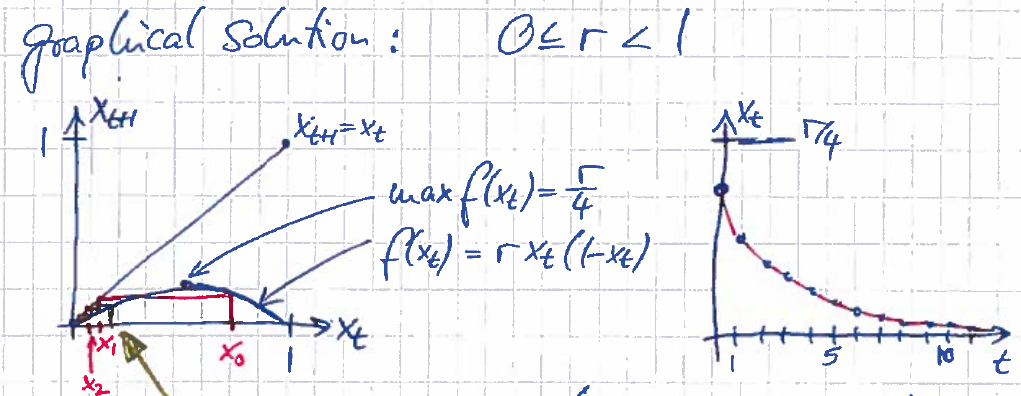
\includegraphics[width=\textwidth]{week7/graphical-solution}\\
    \caption{}
    \label{fig:graphical-solution}
\end{figure}

\begin{framed}
\textbf{Linear stability analysis}
\begin{align}
x_{t+1}&=x^*+\delta x_{t+1} = f(x_t)=f(x^*+\delta x_t)\\
&\approx f(x^*) + f'(x^*)\delta x_t 0 + \cdots
\end{align}
Perturbations are only kept up to first order (linearization). Quadratic and higher order terms are neglected.
\begin{equation}
\biggm\vert\frac{\delta x_{t+1}}{\delta x_{t}}\biggm\vert=|f'(x^*)|
\end{equation}
\begin{align}
|f'(x^*)|<1&:\quad |\delta x_t|=|f'(x^*)|^t|\delta x_0|=e^{\lambda t}|\delta x_0 \\
|f'(x^*)|>1&:\quad  |\delta x_t|=e^{\lambda t}|\delta(x_0)|
\end{align}
\end{framed}


\begin{align}
f(x) &= rx(1-z) \\
\leadsto
f'(x) &= r[(1-x)-x]=r(1-2x) \\
\leadsto
|f'(x^*=0)|&=r\\
\leadsto
x^* &= 0
\end{align}
Stable fixed point for $r<1$. Unstable fixed point for $r>1$.

\textbf{Question:} what happens for $r>1$?
\begin{figure}[h]
    \centering
    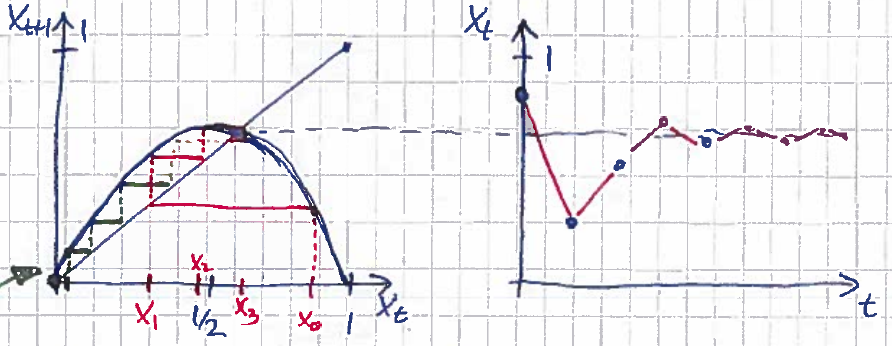
\includegraphics[width=\textwidth]{week7/linear-stability}\\
    \caption{}
    \label{fig:linear-stability}
\end{figure}

Fixed points:
\begin{align}
x^* &= f(x^*) = rx^*(1-x^*)\\
\leadsto
x_0^*=0\ &,\quad x_1^* = \frac{r-1}{r}
\end{align} 

Stability:
\begin{equation}
f'(x_0^*) = r>1
\end{equation}
which means that $x_0^*$ is an unstable fixed point.

\begin{equation}
|f'(x_1^*)|=\biggm\vert r\left(1-2\frac{r-1}{r}\right)\biggm\vert=|2-r|
\end{equation}

\begin{equation}
|f'(x_1^*)| < 1 \Rightarrow 1<r<4
\end{equation}
which means that $x_1^*$ is a stable fixed point.

\textbf{Question:} what happens for $r>3$?

\begin{figure}[p]
    \centering
    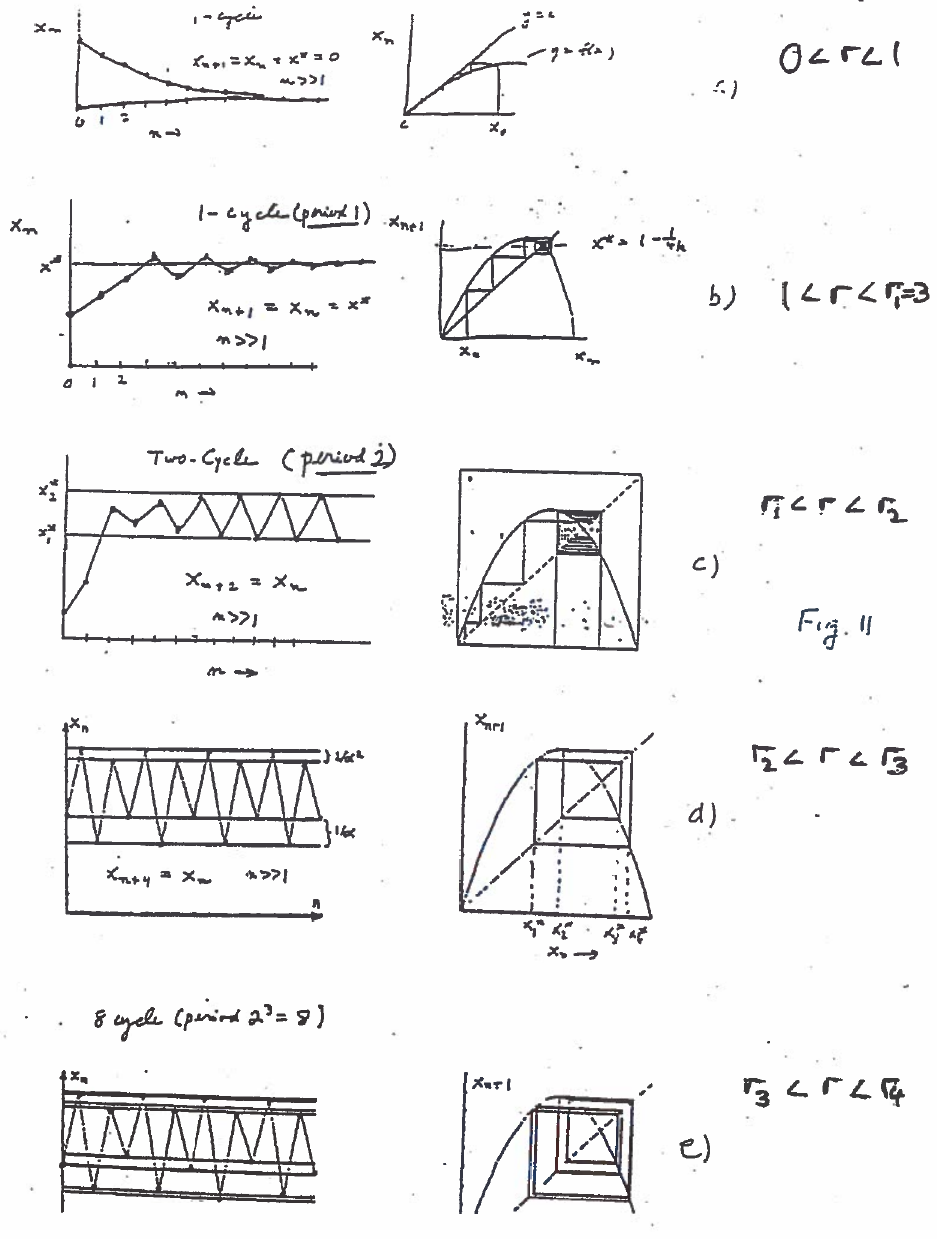
\includegraphics[width=\textwidth]{week7/linear-stability-2}\\
    \caption{}
    \label{fig:linear-stability-2}
\end{figure}

\begin{framed}
two cycle $(r_1=3<r<r_2=?)$: jumps between two values $x_1^*$ and $x_2^*$.

\begin{align}
x_2^*=f(x_1^*)\ &,\quad x_1^*=f(x_2^*) \\
\leadsto
x_2^* = f(f(x_2^*))\, &,\quad x_1^*=f(f(x_1^*))
\end{align}

\begin{align}
f^{(2)}(x) &= f(f(x)) = rf(x)(1-f(x))\\
&= r^2x(x-1)[1-rx(1-x)]
\end{align}

\begin{equation}
\biggm\vert\diff{f^{(2)}(x)}{x}\biggm\vert<1 \Rightarrow r_1=3<r<r_2=?
\end{equation}
stable two-cycle
\end{framed}

\begin{framed}
$r_2<r<r_3$ is a stable four-cycle
\begin{align}
f^{(4)}(x)&=f(f(f(f(x))))\\
\biggm\vert\diff{f^{(4)}(x)}{x}\bigg\vert&<1
\end{align}
\end{framed}
\begin{equation}
3<r\leq r_\infty = 3.57...
\end{equation}
2-cycle, 4-cycle, 8-cycle, ...

\begin{figure}[h]
    \centering
    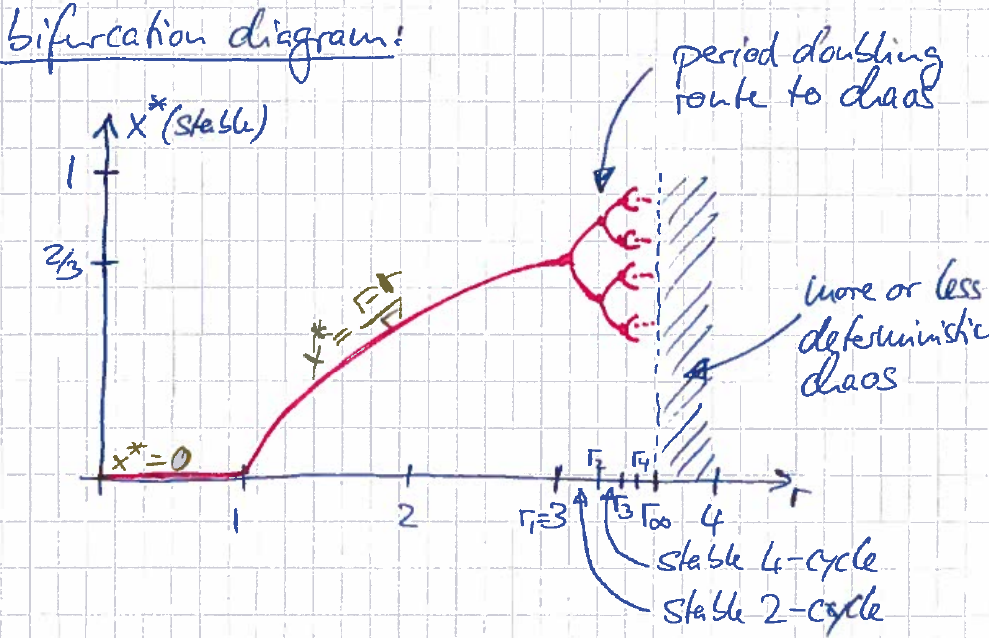
\includegraphics[width=\textwidth]{week7/bifurcation}\\
    \caption{}
    \label{fig:bifurcation}
\end{figure}

\begin{equation}
3.57... \leq r \leq 4
\end{equation}
Mostly chaotic.

\newpage
\textbf{Question:} how can we characterize deterministic chaos?

Liapunov exponent:

\begin{figure}[h]
    \centering
    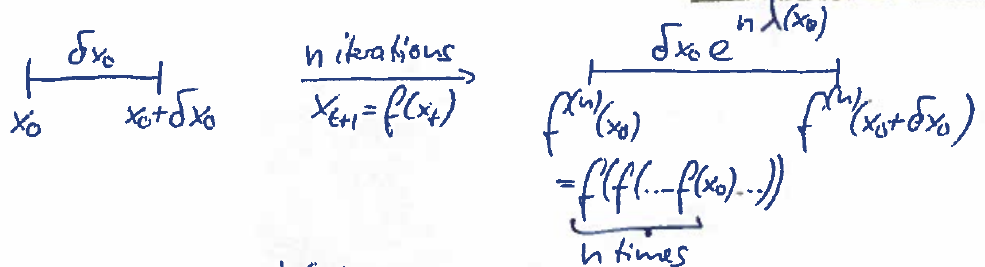
\includegraphics[width=\textwidth]{week7/liapunov}\\
    \caption{}
    \label{fig:liapunov}
\end{figure}

\begin{equation}
\delta x_0e^{n\lambda(x_0)}=|f^{(n)}(x_0+\delta x_0)-f^{(n)}(x_0)|
\end{equation}

\begin{align}
\lambda(x_0) &= \lim_{n\rightarrow\infty}\lim_{\delta x_0\rightarrow0}\frac{1}{n}\ln \biggm\vert \frac{f^{(n)}(x_0+\delta x_0-f^{(n)}(x_0)}{\delta x_0} \\
&= \lim_{n\rightarrow\infty}\frac{1}{n}\ln|(f^{(n)}(x_0))'|\\
&= \lim_{n\rightarrow\infty}\frac{1}{n}\ln|f'(x_{n-1})\cdot f'(x_{n-2})\cdot ... \cdot f'(x_{1})\cdot f'(x_{0})|
\end{align}

\begin{equation}
\lambda(x_0)=\lim_{n\rightarrow\infty}\frac{1}{n}\sum_{i=0}^{n-1}\ln|f'(x_i)|
\end{equation}

Attractive stable limit cycle (with period $T=m$)
\begin{equation}
\lambda(x_0)=\frac{1}{m}\sum_{i=0}^{m-1}\ln|f'(x_i^*)|<0
\end{equation}

Neighboring phase space trajectories with nearly identical initial conditions converge towards each other.

Deterministic chaos:
\begin{equation}
\lambda(x_0)>0
\end{equation}
neighboring trajectories diverge
\begin{figure}[h]
    \centering
    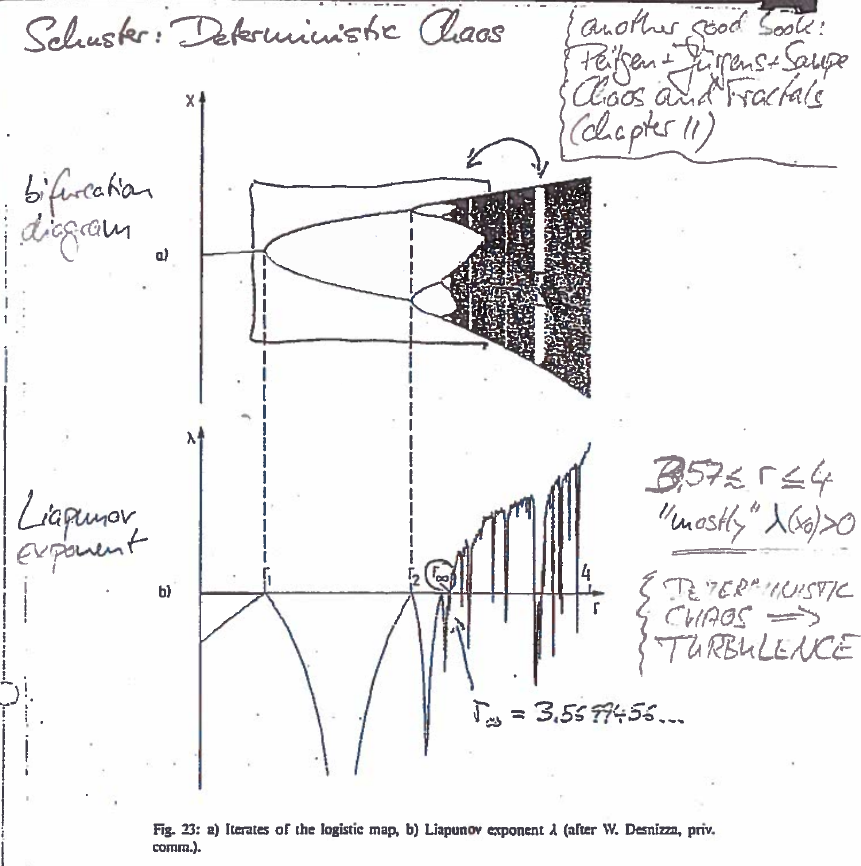
\includegraphics[width=.8\textwidth]{week7/chaos}\\
    \caption{}
    \label{fig:chaos}
\end{figure}

\textbf{Special case (of the logistic map):} $r=4$

Observation: $\lambda(x_0)>0$ leads to divergence of neighboring trajectories. All values $0\leq x_t\leq 1$ occur (as $t$ runs its course).

\textbf{Question:} what is the probability density for a specific x-value?

\begin{equation}
x_{t+1} = 4x_t(1-x_t)
\end{equation}
Substitution:
\begin{equation}
x_t=\frac{1}{2}[1-\cos(2\pi y_t)]
\end{equation}

\begin{align}
t_{t+1} &= \frac{1}{2}[1-\cos(2\pi y_{t+1})] = 4x_t(1-x_t) \\
&= \frac{4}{2}[1-\cos(2\pi y_{t})]\left[1-\frac{1}{2}+\frac{1}{2}\cos(2\pi y_t)\right]\\
&= [1-\cos(2\pi y_{t})][1+\cos(2\pi y_{t})]\\
&= 1-\cos^2(2\pi y_t \\
&=\frac{1}{2}+\frac{1}{2}[\sin^2(2\pi y_t)+\cos^2(2\pi y_t)]-\cos^2(2\pi y_t)\\
&= \frac{1}{2}+\frac{1}{2}[\sin^2(2\pi y_t)-\cos^2(2\pi y_t)]\\
&= \frac{1}{2}[1-\cos(4\pi y_t)]
\end{align}

Solution:
\begin{equation}
y_{t+1} = 2y_t\ ,\quad 0\leq y_t \leq 1
\end{equation}
\begin{equation}
y_t = 2^ty_0
\end{equation}

\begin{figure}[h]
    \centering
    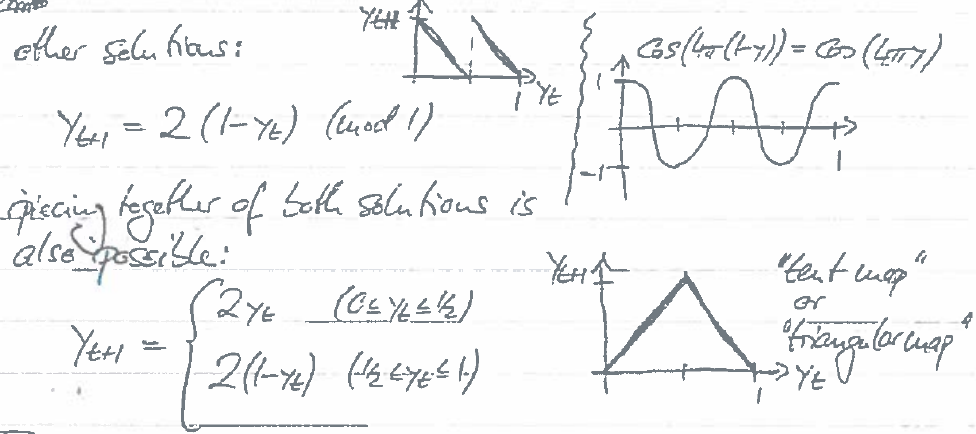
\includegraphics[width=\textwidth]{week7/other-solution}\\
    \caption{}
    \label{fig:other-solution}
\end{figure}

\begin{framed}
Once again: sensitive dependence on initial conditions

\begin{equation}
y_0 = \alpha_12^{-1} + \alpha_22^{-2} + \alpha_32^{-3} + \dots = \sum_{i=1}^\infty\alpha_i2^{-i}
\end{equation}

\begin{align}
y_1 &= 2y_0 \\
&= \alpha_22^{-2} + \alpha_32^{-3} + \alpha_42^{-4}+\dots\\
&= \sum_{i=1+1}^\infty\alpha_{i+1}2^{-i}
\end{align}

\begin{align}
y_2 &= \dots = \sum_{i=1+1}^\infty\alpha_{i+2}2^{-i}\\
&\vdots\\
y_t &= \sum_{i=1+1}^\infty\alpha_{i+t}2^{-i}
\end{align}

\begin{align}
y_0 &= 0.\alpha_1\alpha_2\dots\alpha_n\alpha_{n+1}\dots\\
y_0' &= 0.\alpha_1\alpha_2\dots\alpha_n\alpha_{n+1}'\dots 
\end{align}

\begin{equation}
|y_0-y_0'|\leq \underbrace{0.00\dots01}_{(n-1)\ \mathrm{times}} = \frac{1}{2^n}
\end{equation}
During the first $n$ time steps the two trajectories $y_i=f^{(i)}(y_0)$ and $y_i'=f^{(i)}(y_0')$ stay close together; thereafter they separate completely. Sensitive dependence on initial condition.
\end{framed}

\begin{equation}
y_0=0.\alpha_1\alpha_2\alpha_3\dots=\sum_{i=1}^\infty\alpha_i2^{-i}
\end{equation}
with random numbers $\alpha_i=\{0,1\}$.

$\{y_t=f^{(t)}(y_0)\}$ uniformly distributed on $[0,1]$

\begin{equation}
\rho(y) = \lim_{T\rightarrow\infty}\frac{1}{T}\sum_{t=0}^{T-0}\delta(y-y_t) = \begin{cases}
1,\quad 0\leq y \leq 1 \\ 0, \quad \mathrm{else} \end{cases}
\end{equation}

\begin{figure}[h]
    \centering
    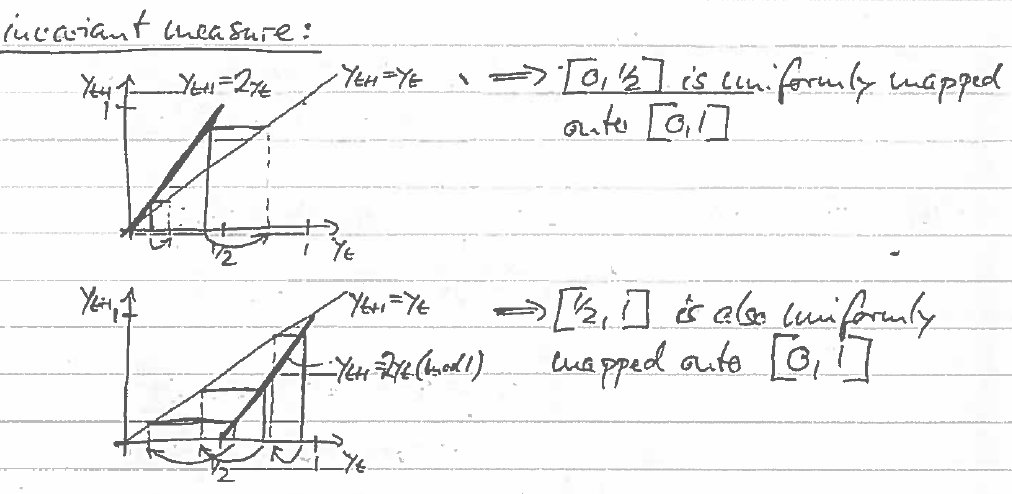
\includegraphics[width=\textwidth]{week7/invariant-measure}\\
    \caption{}
    \label{fig:invariant-measure}
\end{figure}

Back to our original question:

\begin{align}
1 &= \int_0^1\rho(y) dy = \int_0^1dy=2\int_0^\frac{1}{2}dy\\
&= 2\int_0^1\frac{dx}{\pi\sin(2\pi y)} = \frac{2}{\pi}\int_0^1\frac{dx}{\sqrt{1-\cos^2(2\pi y)}}\\
&= \frac{2}{\pi}\int_0^1\frac{dx}{[1-(1-2x)^2]^{1/2}} = \frac{2}{\pi}\int_0^1\frac{dx}{[4x-4x^2]^{1/2}} = \int_0^1\frac{1}{\pi[x(1-x)]^{1/2}}dx
\end{align}

\begin{equation}
\rho(x) = \frac{1}{\pi[x(1-x)]^{1/2}}
\end{equation}
invariant measure for the map $x_{t+1} = 4x_t(1-x_t)$.

Transparency:
\begin{align}
\rho(x)\ ,&\quad x_{t+1}=4x_t(1-x_t)\\
\rho(v)\ ,&\quad v_{t+1}=1-2v_t^2
\end{align}

\begin{figure}[h]
    \centering
    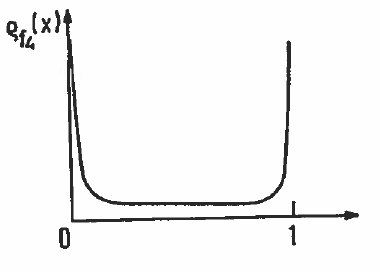
\includegraphics[width=.5\textwidth]{week7/invariant-density}\\
    \caption{}
    \label{fig:invariant-density}
\end{figure}
\begin{figure}[h]
    \centering
    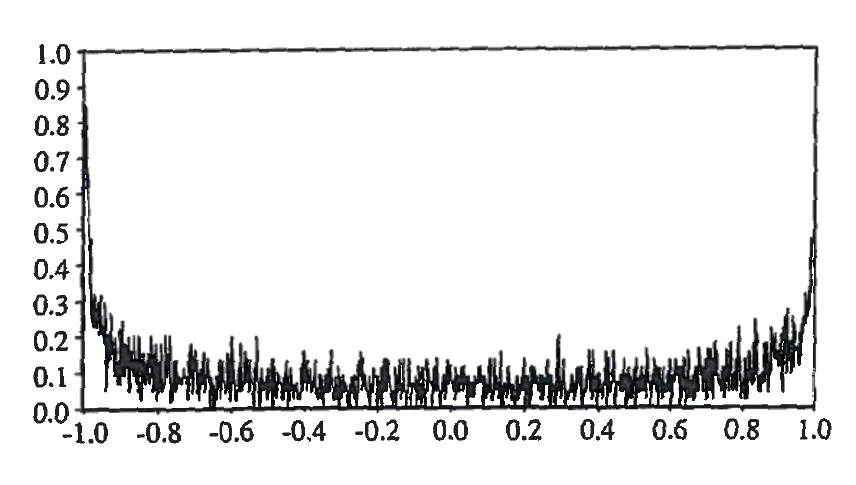
\includegraphics[width=.8\textwidth]{week7/norm-hist}\\
    \caption{}
    \label{fig:norm-hist}
\end{figure}

\newpage
\begin{shaded}
I left out the last lecture on turbulence, pages: 106-112.
\end{shaded}